\section{Serial Accessories}

\subsection{\acs{USB}-C serial adaptor}

% Serial accessories attach to the x-IMU3 using a \acs{USB}-C serial adaptor.
The \acs{USB}-C serial adaptor, shown in \fref{fig:usbCSerialAdapter}, allows serial connections to be made through the \acs{USB}-C socket.  The adaptor provides access to \ac{TX}, \ac{RX}, and ground connections through a \ac{TRS} socket as described in \fref{tab:trsConnections}.  Serial accessories typically do not expect to receive data from the x-IMU3 and so can use the idle-high \ac{TX} output as a 3.3 V power supply.

\begin{figure}[H]
    \centering
    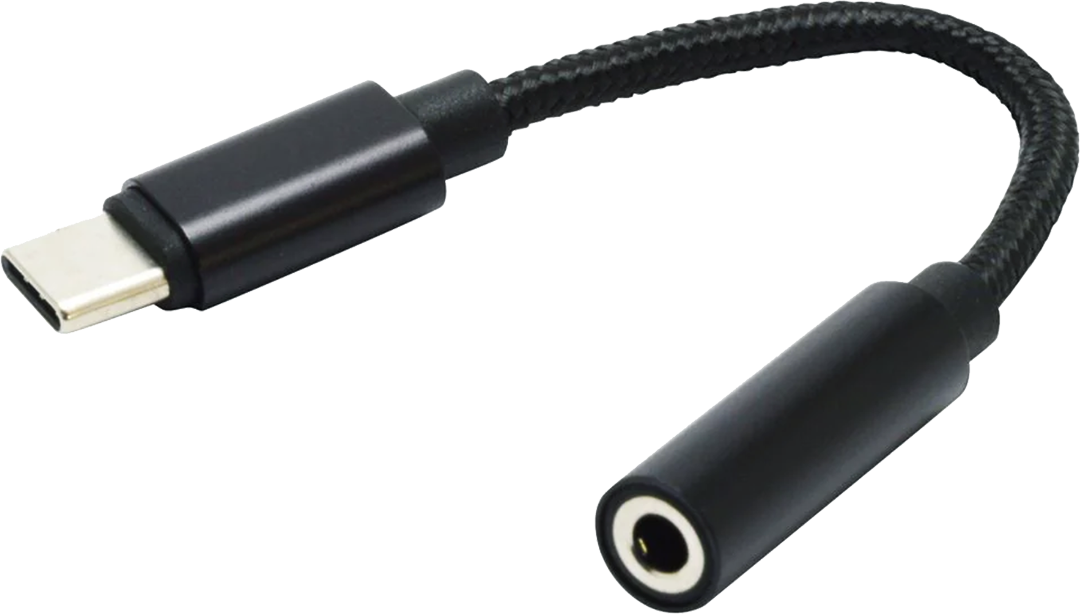
\includegraphics[width=0.3\textwidth]{Images/saAdapter.png}
    \caption{\acs{USB}-C serial adaptor}
    \label{fig:usbCSerialAdapter}
\end{figure}

\customTable
{l l}
{\ac{TRS} & Connection}
{
    Tip & Serial \ac{RX}\\
    Ring & Serial \ac{TX} / 3.3 V output\\
    Sleeve & Ground\\
}
{\acs{USB}-C serial adaptor \ac{TRS} connections}
{tab:trsConnections}

The \acs{USB}-C serial adaptor is also available with a \acs{USB}-C power input, as shown in \fref{fig:usbCSerialAdapterWithPower}.  This allows the x-IMU3 to be powered by \ac{USB} while using a \acs{USB}-C serial adaptor.  This provides \ac{USB} power only.  Normal \ac{USB} communication is not possible when using a \acs{USB}-C serial adaptor.

\begin{figure}[H]
    \centering
    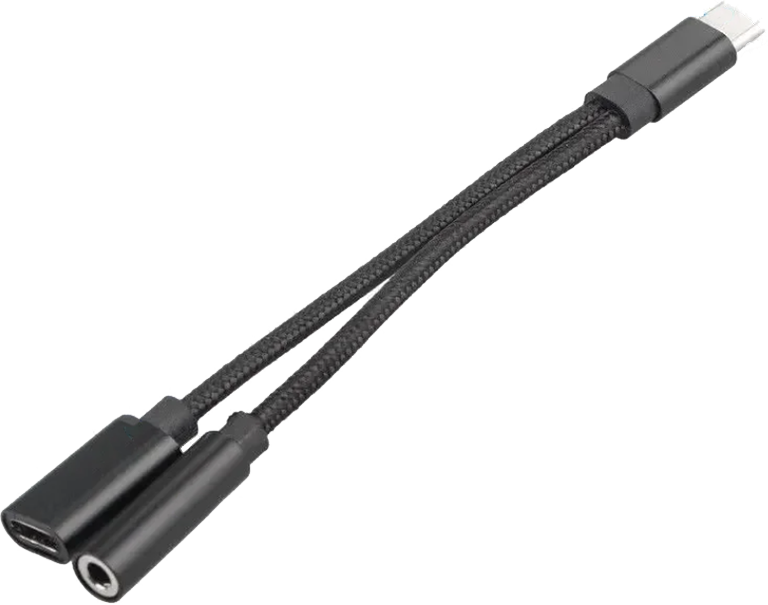
\includegraphics[width=0.4\textwidth]{Images/saAdapterWithPower.png}
    \caption{\acs{USB}-C serial adaptor with power}
    \label{fig:usbCSerialAdapterWithPower}
\end{figure}

\newcommand{\specificationTable}[4]{
    \customTable
    {l c c}
    {Characteristic & Value & Notes}
    {
        #1
    }
    {#2}
    {#3}
    \textbf{Notes}
    \begin{enumerate}[nolistsep]
        #4
    \end{enumerate}
}

\newcommand{\messageExample}[1]{
    \begin{table}[H]
        \def\arraystretch{1.5}
        \begin{tabular}{l l}
            \textbf{Example:} & \texttt{#1\textbackslash n}
        \end{tabular}
    \end{table}
}

\subsection{x-IMU3-SA-A2}

The x-IMU3-SA-A2 is a 2-channel analogue input for interfacing to analogue sensors such as ...., and ...
%
Power external electronics.
%
% The x-IMU3-SA-A2 connects to the x-IMU3 through the \acs{USB}-C serial adaptor.

\begin{figure}[H]
    \centering
    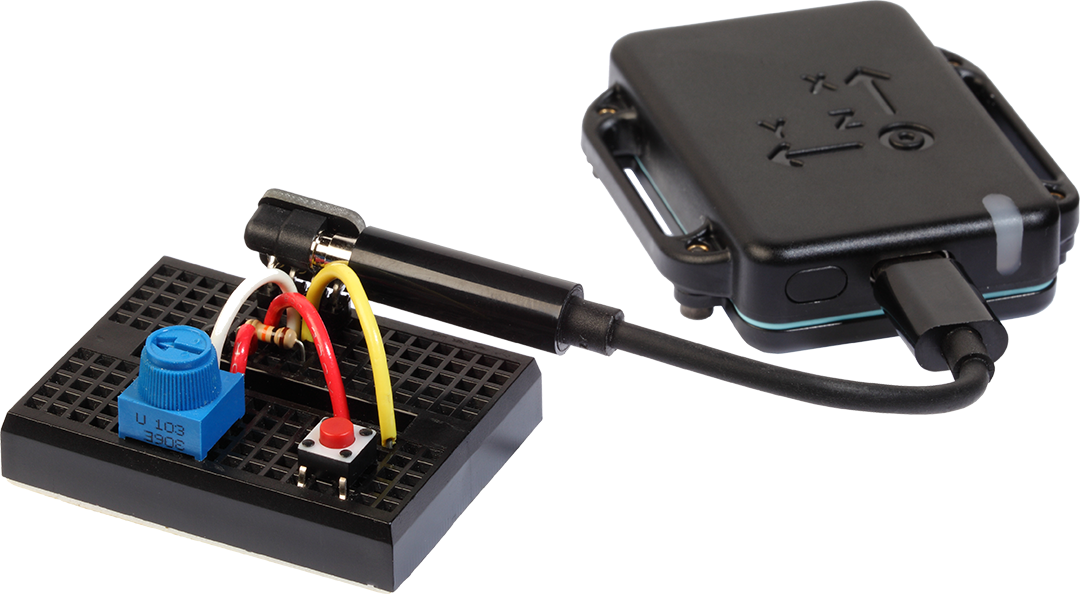
\includegraphics[width=0.5\textwidth]{Images/saA2.png}
    \caption{x-IMU3-SA-A2}
    \label{fig:ximu3SAA2}
\end{figure}

\subsubsection{Technical specification}

\specificationTable
{
    Number of analogue inputs & 2 & \ref{itm:ximu3SAA2Specification1}\\
    Analogue input resolution & 8-bit & \ref{itm:ximu3SAA2Specification2}\\
    Analogue input range & 0 V to 3.3 V & \ref{itm:ximu3SAA2Specification3}\\
    Sample rate & 100 Hz & \ref{itm:ximu3SAA2Specification4}\\
    \acs{UART} baud rate & 115200 & -\\
}
{x-IMU3-SA-A2 specification}
{tab:ximu3SAA2Specification}
{
    \item \label{itm:ximu3SAA2Specification1} This is a note
    \item \label{itm:ximu3SAA2Specification2} This is a note
    \item \label{itm:ximu3SAA2Specification3} Analogue input pins are 5 V tolerant
    \item \label{itm:ximu3SAA2Specification4} The sample rate accuracy is not specified.  Applications that require precise timing should not infer timing from the nominal sample rate and should instead use the timestamp of each measurement.
}

\subsubsection{Hardware}

% y = -1.6
% xStart = -3.4
% xWidth = 0.74

% for counter in range(4):
%     x = xStart + (xWidth * counter)
%     pin = counter + 1
%     print("        \\node[annotation] at (" + "{:.2f}".format(x) + "," + "{:.2f}".format(y) + ") {\\ref{itm:ximu3SAA2" + str(pin) + "}};")

\begin{figure}[H]
    \centering
    \begin{tikzpicture}[annotation/.style={draw=black, fill=white, very thick, minimum size=6mm}]
        \node at (0,0) {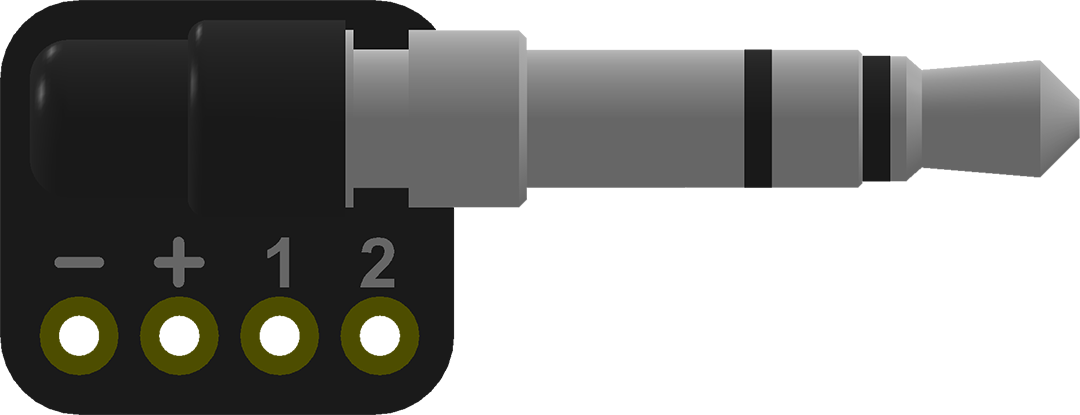
\includegraphics[width=0.5\textwidth]{Images/saA2Top.png}};
        \node[annotation] at (-3.40,-1.60) {\ref{itm:ximu3SAA21}};
        \node[annotation] at (-2.66,-1.60) {\ref{itm:ximu3SAA22}};
        \node[annotation] at (-1.92,-1.60) {\ref{itm:ximu3SAA23}};
        \node[annotation] at (-1.18,-1.60) {\ref{itm:ximu3SAA24}};
    \end{tikzpicture}
    \caption{x-IMU3-SA-A2 Top}
    \label{fig:ximu3SAA2Top}
\end{figure}

\begin{figure}[H]
    \centering
    \begin{tikzpicture}[annotation/.style={circle, draw=black, fill=white, very thick, minimum size=7mm}]
        \node at (0,0) {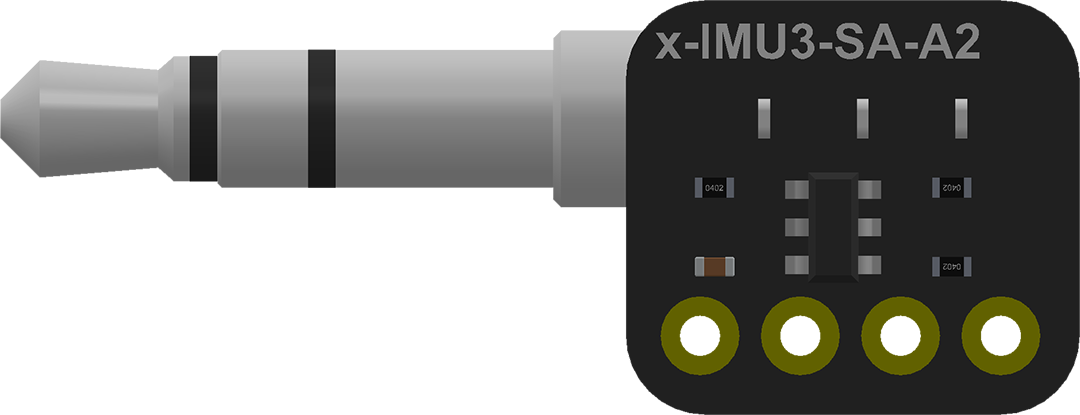
\includegraphics[width=0.5\textwidth]{Images/saA2Bottom.png}};
        \node[annotation] at (-0.7,0.67) {\ref{itm:ximu3SAA25}};
    \end{tikzpicture}
    \caption{x-IMU3-SA-A2 Bottom}
    \label{fig:ximu3SAA2Bottom}
\end{figure}

\begin{enumerate}
    \item \label{itm:ximu3SAA21} Ground
    \item \label{itm:ximu3SAA22} 3.3 V output
    \item \label{itm:ximu3SAA23} Channel 1 input
    \item \label{itm:ximu3SAA24} Channel 2 input
    \item \label{itm:ximu3SAA25} \ac{TRS} jack
\end{enumerate}

\vskip 2em

\warning{Electrical connections require basic soldering skills.}

\subsubsection{Communication protocol}

Analogue input measurements are streamed continuously at the fixed sample rate as two comma-separated values terminated by a \ac{LF} control character.  Each value is a voltage rounded to two decimal places.

\messageExample{1.23,2.34}
